\section{Durchführung}
\label{sec:Durchführung}
In diesem Versuch werden, wie im \autoref{sec:Ziel} beschrieben, die Trägheitsmomente verschiedener Körper berechnet. 

\subsection{Vorbereitungsaufgaben}
\label{subsec:D_Va}
Vorbereitend zu diesem Versuch werden zunächst ein paar beispielhafte Drehmomente $M_{\text{Bsp}}$
zu verschiedenen Abständen $r_{\text{Bsp}}$ berechnet. Dazu wird die Formel $M = Fr\, \text{cos}(\frac{\pi}{2})$ genutzt. Die errechneten Werte können \autoref{tab:D_VA} entnommen werden.
\begin{table}
    \centering
    \caption{Berechnete Werte der Vorbereitungsaufgabe} 
    \label{tab:D_VA}
    \begin{tabular}{c c}
        \toprule
        $r_{\text{Bsp}}\mathrm{/} \unit{\centi\metre}$ & $M_{\text{Bsp}}\mathrm{/}\unit{{\milli\newton\metre}}$\\
        \midrule
        5 & 3.563 \\
        7.5 & 5.3 \\
        10 & 7.07 \\
        12.5 & 8.8 \\
        15 & 10.6 \\
        17.5 & 12.37 \\
        20 & 14.14 \\
        22.5 & 15.9 \\
        25 & 17.67 \\
        \bottomrule 
    \end{tabular}
\end{table}
\subsection{Experimentelle Bestimmung der Apparatkonstanten}
\label{subsec:D_const}
Zu Beginn werden die Winkelrichtgröße $D$ und das Eigenträgheitsmoment $I_D$ der Drill-Achse bestimmt. Dazu wird zunächst ein Stab durch die Drill-Achse gesteckt. Dann wird ein Newtonmeter, mit einem 
Winkel von $90\unit{\degree}$, an dem Stab eingehängt. Die Drill-Achse wird nun mit dem Newtonmeter um $90\unit{\degree}$ gedreht. Dann wird die Kraft auf dem Newtonmeter abgelesen und notiert. Diese 
Messung wird mindestens zehn mal durchgeführt und die Ergebnisse danach gemittelt. Dazu wird ebenfalls der Abstand der Aufhängung zur Drill-Achse notiert. Daraus wird die Winkelrichtgröße 
bestimmt. Um das Eigenträgheitsmoment der Drill-Achse zu bestimmen werden zwei Gewichte in symetrischen Abständen an der Stange angebracht. Nun wird die Stange ausgelenkt, sodass sie schwingt.
Dabei wird die Schwingungsdauer für mehrere Perioden gemessen und schließlich gemittelt. Diese Messung wird für mindestens zehn verschiedene Aufhängungen der Gewichte durchgeführt, wobei der Abstand
der Gewichte zum Mittelpunkt ebenfalls notiert wird. Aus dieser Messung kann dan das Eigenträgheitsmoment bestimmt werden.
\subsection{Experimentelle Bestimmung der Trägheitsmomente einfacher Körper}
\label{subsec:D_Körper}
Es soll nun das Trägheitsmoment zweier einfacher Körper bestimmt werden. Dazu werden diese Körper zunächst gewogen und abgemessen. Dann werden die Körper auf der Drill-Achse angebracht. Nun werden
die Körper um $90\unit{\degree}$ auf der Drill-Achse ausgelenkt. Es wird die Schwingungsdauer gemessen. Pro Körper werden fünf Messungen durchgeführt und die Ergebnisse werden gemittelt.
\subsection{Experimentelle Bestimmung der Trägheitsmomente komplexer Körper}
\label{subsec:D_Figur}
Zuletzt werden noch die Trägheitsmomente komplexerer Körper bestimmt. Dazu wird erneut eine Drill-Achse genutzt. Als komplexer Körper wird eine Holzpuppe verwendet. Diese ist in \autoref{fig:D_subfig} zu sehen.

\begin{figure}
    \centering
    \caption{Abbildung zur experimentellen Bestimmung der Trägheitsmomente komplexer Körper:In dieser Abbildung ist eine Stellung der verwendete Holzpuppe auf der Drill-Achse zu sehen.}
    \label{fig:D_subfig}
    \begin{subfigure}{0.48\textwidth}
        \centering
        \caption{Stellung 1}
        \label{fig:D_Holzpuppe1}
        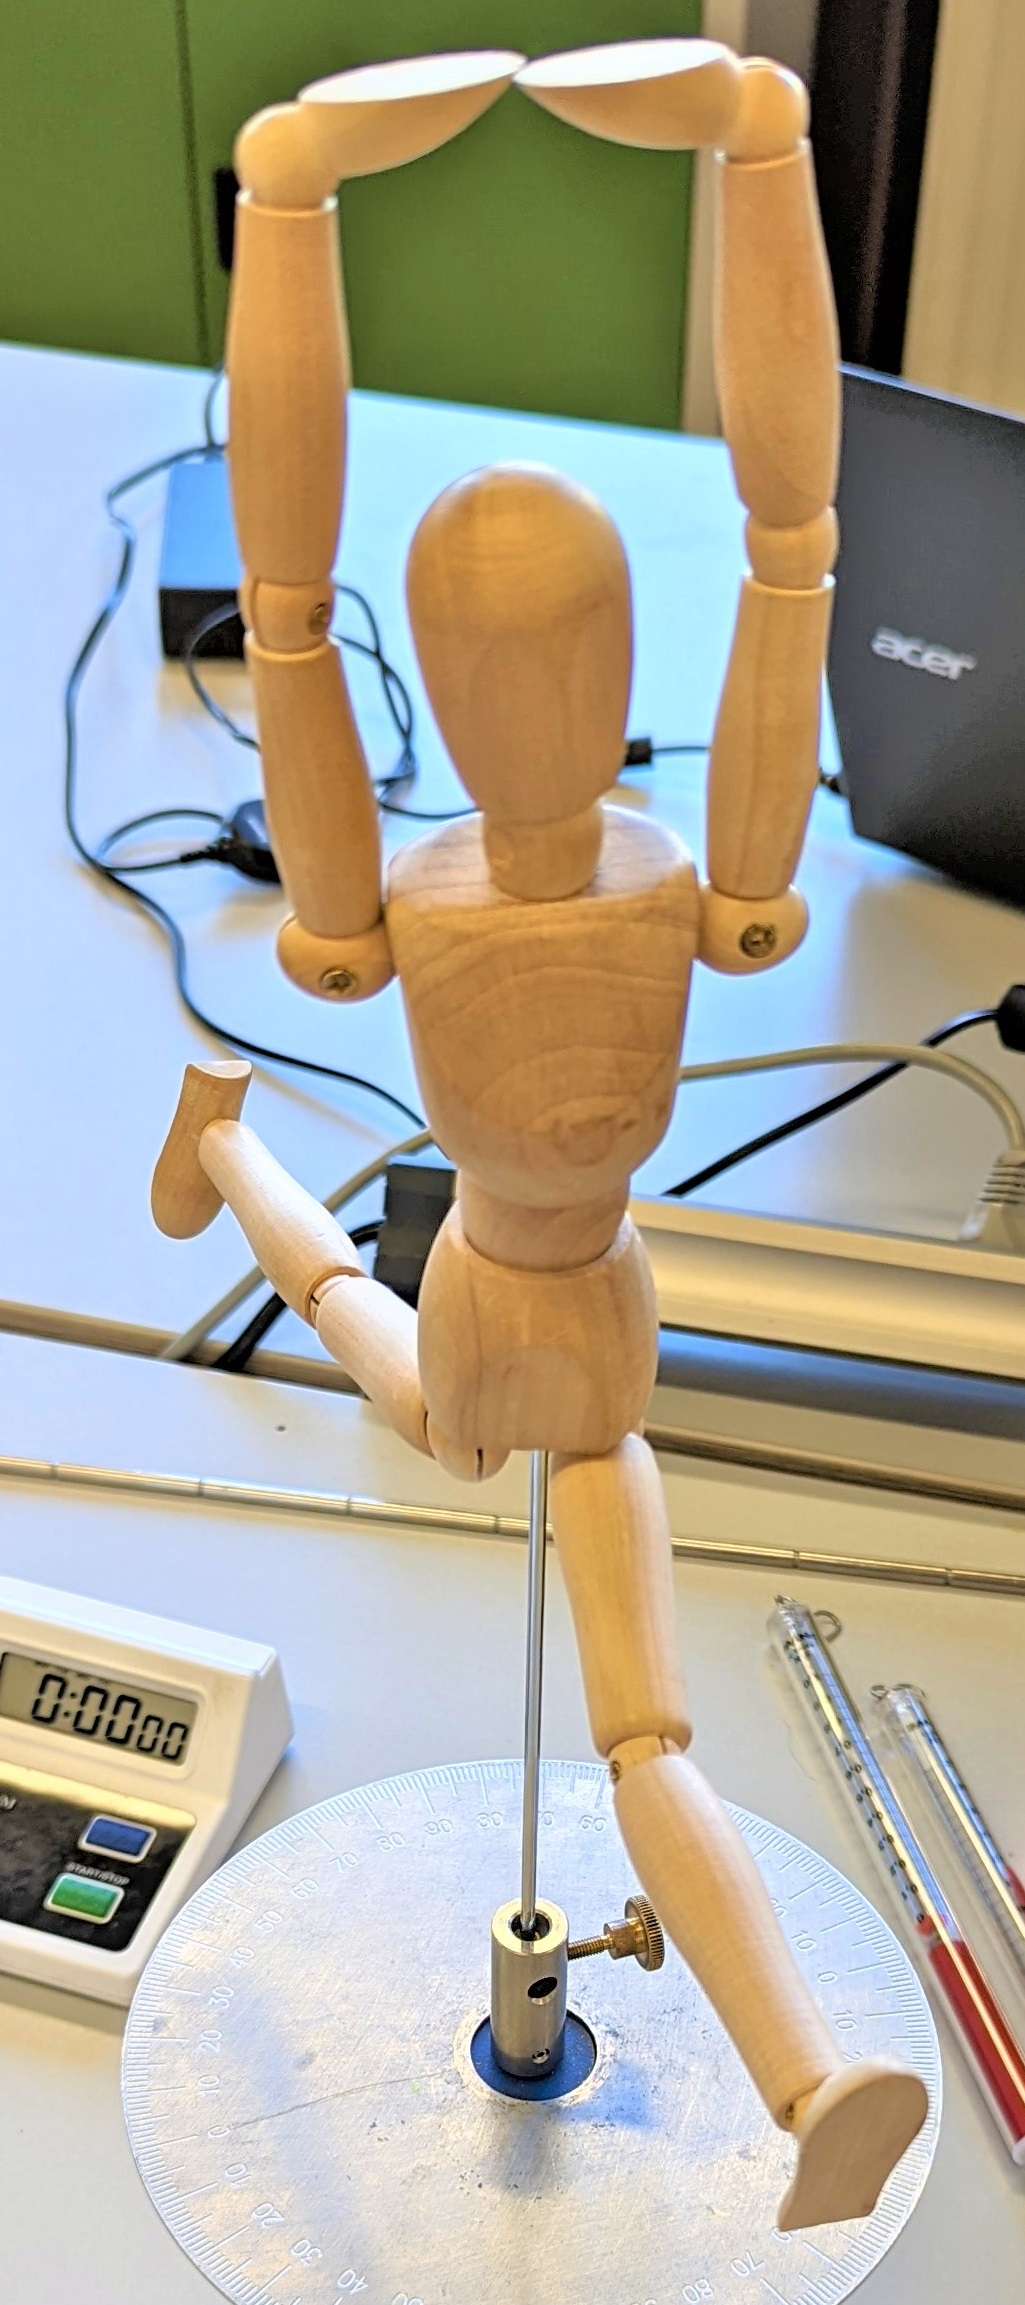
\includegraphics[width=0.6\textwidth]{content/Ballet3.jpg}
    \end{subfigure}
    \hfill
    \begin{subfigure}{0.48\textwidth}
        \centering
        \caption{Stellung 2}
        \label{fig:D_Holzpuppe2}
        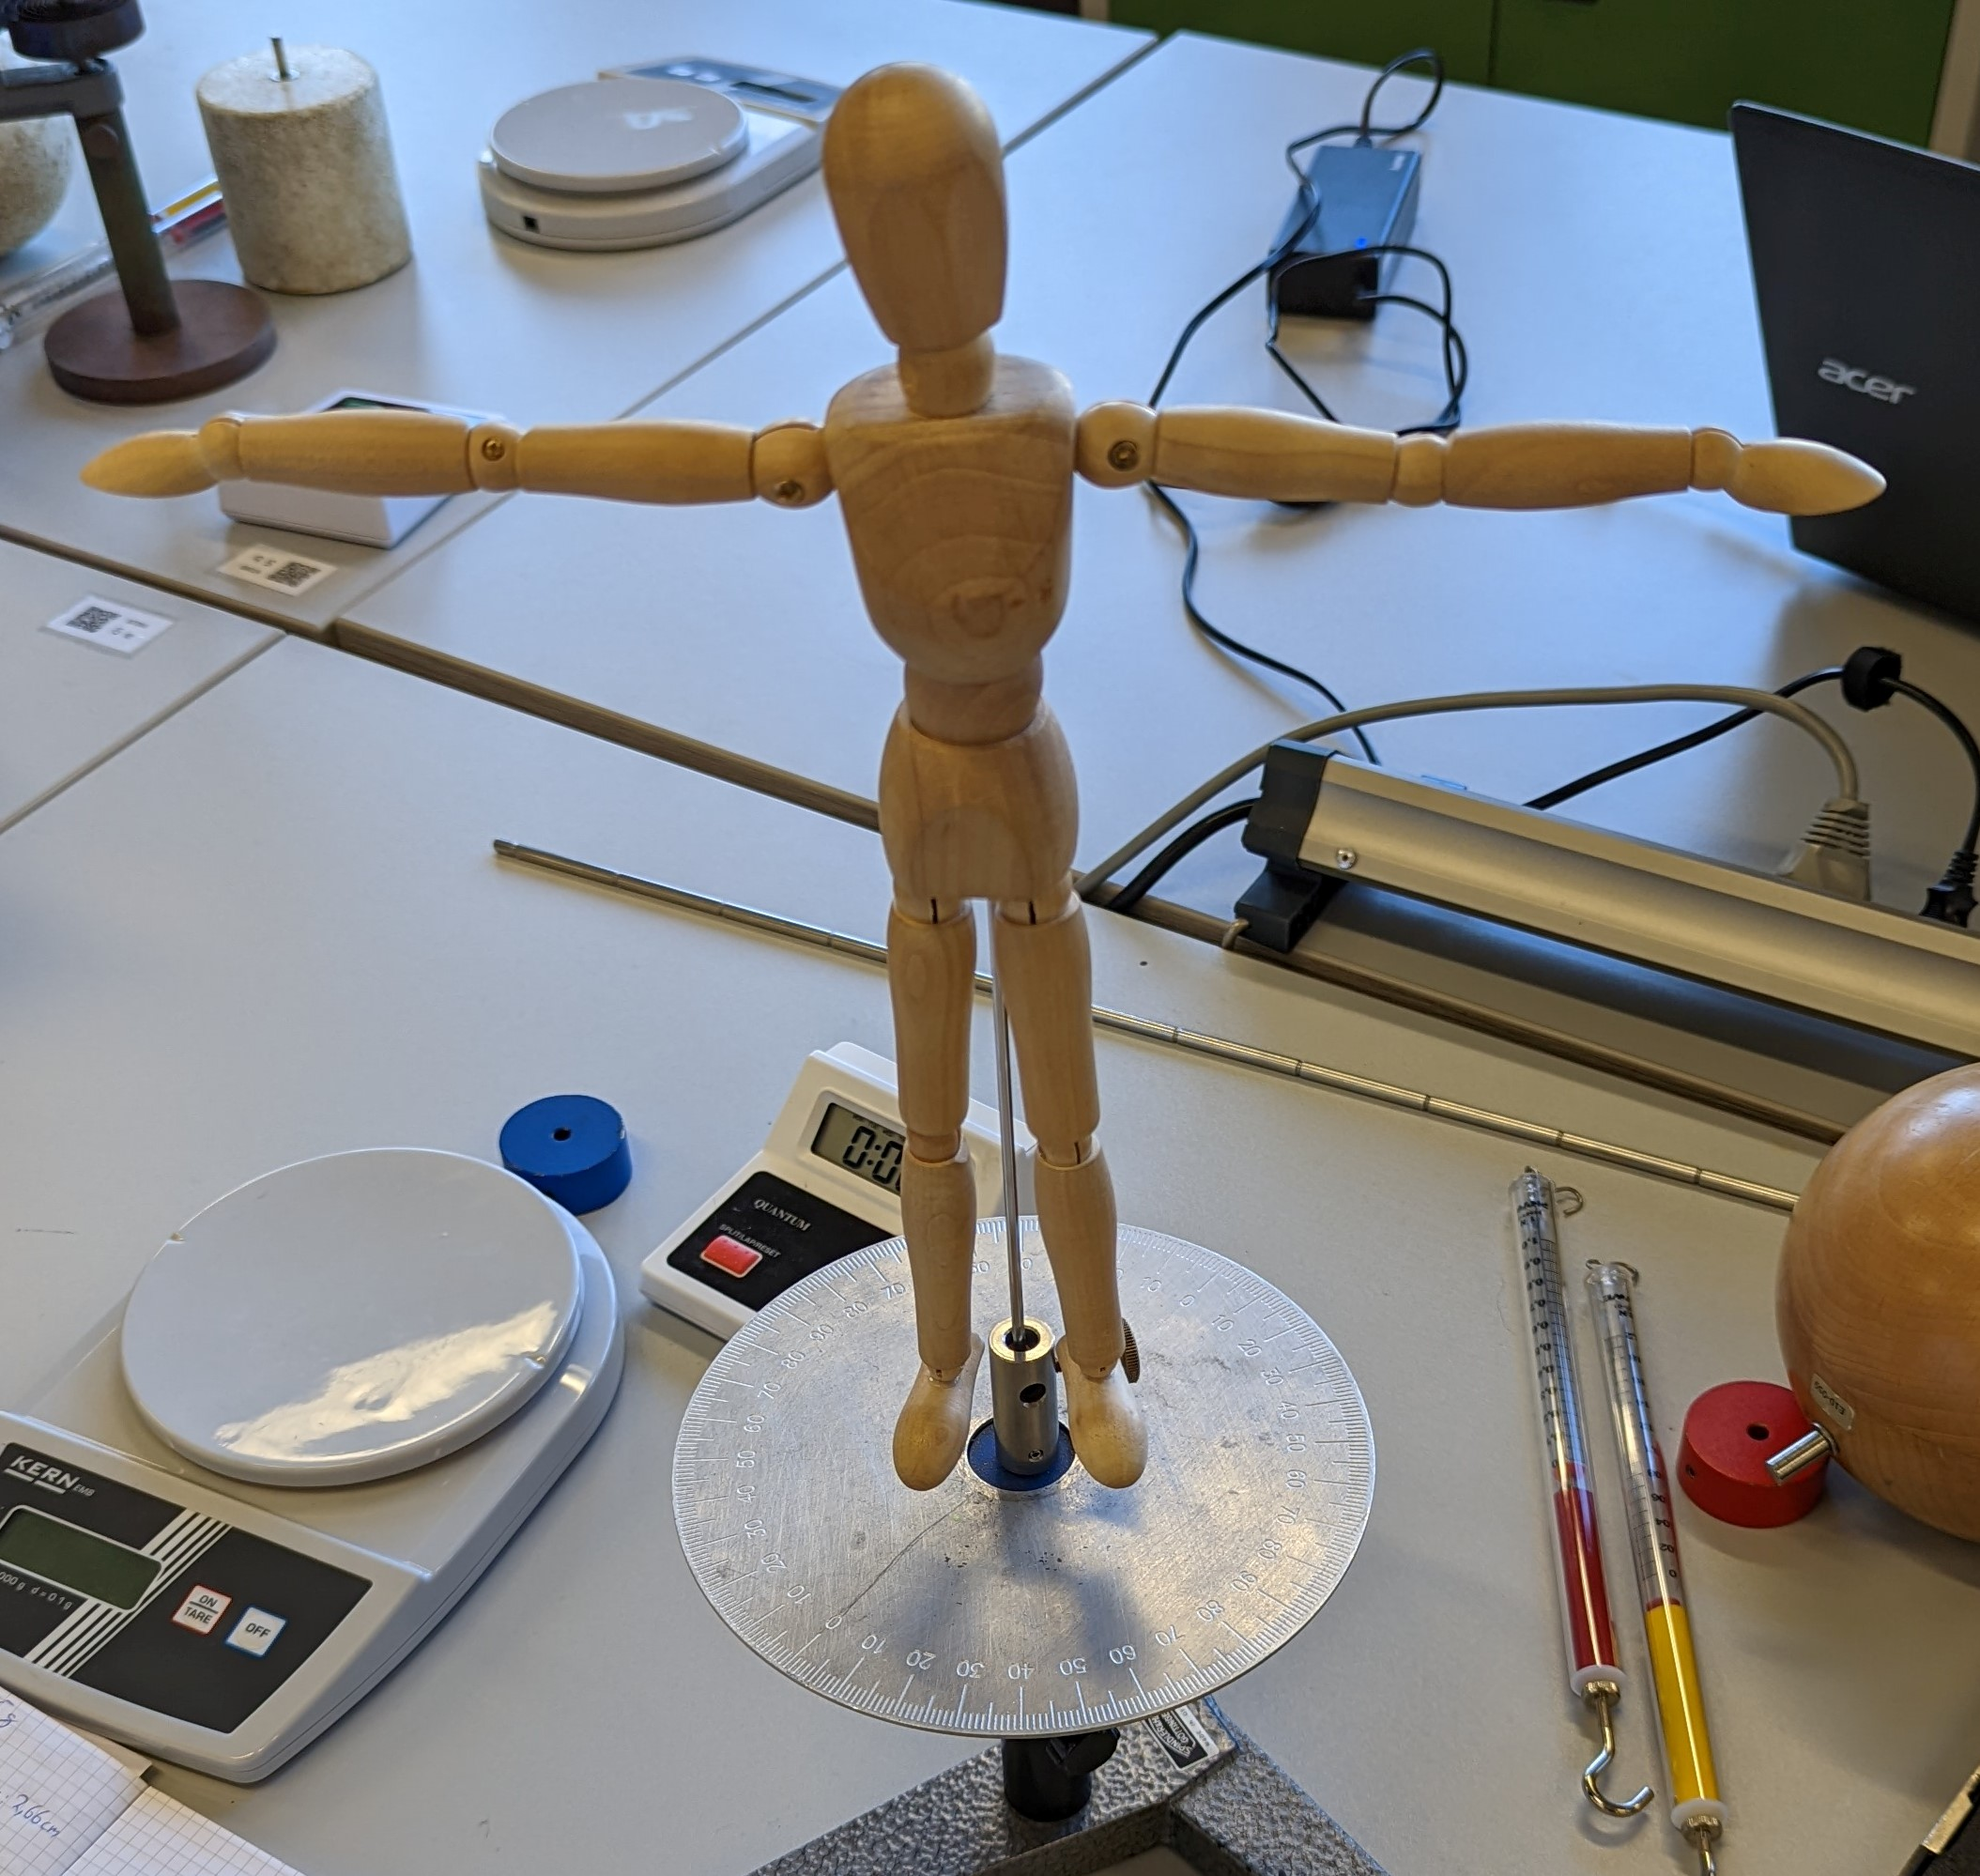
\includegraphics[width=0.8\textwidth]{content/T_Pose3.jpg}
    \end{subfigure}    
\end{figure}

Nun wird die Holzpuppe an ihrem Stab in die Drill-Achse eingespannt. Zunächst wird sie in Stellung 1 gebracht, welche in \autoref{fig:D_Holzpuppe1} zusehen ist. In dieser Stellung wird die Figur fünf 
mal um $90\unit{\degree}$ und weitere fünf mal um $120\unit{\degree}$ ausgelenkt. Dabei werden immer circa drei Periodendauern gemessen und abschließend gemittelt. Dieses Verfahren wird für 
Stellung 2, welche \autoref{fig:D_Holzpuppe2} entnommen werden kenn, erneut durchgeführt. 